\section{RoadMap}
	\subsection{RoadMap Inicial}

	O conceito de roadmap está relacionado ao planejamento de release. Uma release pode ser entendido como um período de desenvolvimento com o objetivo de lançar uma nova versão de produto. (LEFFINGWELL, 2010). 

	O roadmap alinha objetivo do time e do programa com os objetivos do negócio e providência visibilidade do projeto ao longo das entregas, dessa forma, torna-se possível obter uma visão ao longo do tempo das entrega de funcionalidades de um produto até a data prevista para o final do projeto (Scaled Agile Framework, 2015).

	Para ser bem sucedido, deve-se efetuar o planejamento do roadmap junto com o cliente e envolvidos, fazendo com que aumente a qualidade da decisão e contribuindo para obtenção do apoio dos envolvidos durante o ciclo de execução do projeto (SCRUMEX, 2011). 					
	Embora roadmap possa ser interpretado como um “plano de intenção”, ele está sujeito a mudanças e deve ser revisado periodicamente ao final de cada release.

	\subsection{RoadMap do Projeto}

	O roadmap inicial foi construído levando em consideração a priorização realizada com a tabela WSJF e conversas com o cliente. Foi definido para esse projeto, duas releases com período de 45 dias cada.

	\begin{figure}[h]
		\centering
		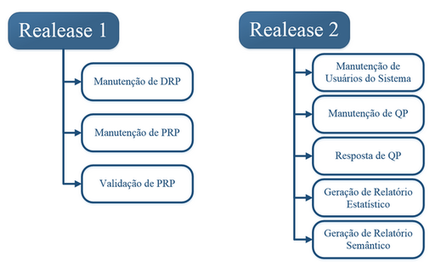
\includegraphics{imagens/roadmap1.png}
		\caption{roadmap}
		\label{imagem}
	\end{figure}